\paragraph{Questions, corpus, and protocol.}
We ask whether completed diagnostics agree with independently executed small-grid semantics, whether residue reduction and the specialized DP change exact-search behavior, and whether a universal envelope is attained on the declared grids. The deterministic generator uses seed 20261003. The effectiveness corpus contains 48 synthetic programs, 12 canonical examples, and six public-rule-derived fragments: 66 programs in total, of which the oracle classifies 50 as sensitive and 16 as safe. The corresponding group counts are 37/48, 8/12, and 5/6 sensitive. Each program has \SmallVarsMin{}--\SmallVarsMax{} tick variables, two to four policies, and 21--1600 input assignments. Counting repeated syntax separately across policies gives \SmallNodesMin{}--\SmallNodesMax{} abstract syntax tree (AST) nodes (median 13); maximum root-to-leaf depth is \SmallDepthMin{}--\SmallDepthMax{} (median 4), with the root counted as depth one. These are small expression benchmarks rather than production programs.

The exhaustive oracle evaluates all 19,940 assignments in this corpus using Python Decimal's six rounding conventions, separately from the analyzer's Fraction quantizer and SMT encoding. Terminating rationals are converted by exact digit-tuple construction, independent of Decimal's current precision. The precision budget includes denominator powers of two and five and intermediate decimal spans. Inexact and rounded arithmetic traps reject silent approximation; only the explicitly requested grid quantization may round. Nonterminating conversions or normalized quantum divisions are rejected. All saved corpus computations complete under these guards. The oracle shares the parsed AST with the analyzer, so this agreement tests arithmetic and analysis after parsing; it does not independently establish every parser translation. Saved \texttt{ground\_truth.json} records each oracle maximum and witness, and \texttt{diagnostics.json} records method outputs.

RoundGuard's automatic dispatch is compared with the same symbolic encoder on the full box, 32 uniformly sampled assignments, Hypothesis search configured with \texttt{max\_examples=64}, and independent range intervals for each policy. Sampling stops at the first differing assignment; Hypothesis may also shrink a found example, so 64 is a configuration parameter rather than a matched wall-time or strict total-evaluation budget. A testing result with no witness does not prove equality. Interval warnings are counted against the exact label, but the interval baseline is a deliberately simple correlation-losing envelope, not a state-of-the-art numerical analyzer. The effectiveness measurements have one execution per program and method; their medians summarize this heterogeneous corpus rather than repeated-run timing uncertainty.

\paragraph{Small-grid agreement and detection.}
\begin{table}[ht]
\centering\begin{tabular}{lrrrrr}
\toprule
Method & Cases & FP & Missed & Unknown & Median ms \\
\midrule
RoundGuard & 66 & 0 & 0 & 0 & 4.32 \\
Full-grid SMT & 66 & 0 & 0 & 0 & 5.92 \\
Random (32) & 66 & 0 & 2 & 0 & 1.00 \\
Hypothesis (64) & 66 & 0 & 1 & 0 & 45.82 \\
Independent intervals & 66 & 15 & 0 & 0 & 0.13 \\
\bottomrule
\end{tabular}
\caption{Effectiveness on 66 programs: 50 sensitive and 16 safe. FP (false positive) counts warnings on oracle-safe programs; Missed counts oracle-sensitive programs without a reported witness or warning. A testing miss is not a false proof of safety. Exact-method maxima also agree with the exhaustive oracle. Median wall times are across programs.}
\label{tab:accuracy}
\end{table}
Both exact methods complete on all 66 programs, match every oracle maximum, and have no false warnings or missed sensitive cases (Table~\ref{tab:accuracy}). Automatic dispatch selects residue DP for 22 programs, reduced SMT for 19, and unreduced SMT for 25. Its median wall time is \AutoMedian\,ms, compared with \SMTMedian\,ms for full-grid SMT. Random testing misses two threshold programs, and Hypothesis misses one currency-conversion program. Independent intervals warn on 15 of the 16 safe programs. These results establish agreement on the saved cases; neither the mixture nor the small miss counts estimates defect prevalence in financial software.

\paragraph{Scaling and method ablations.}
The scaling suite has 24 independent-line cases: $n\in\{2,4,8,16,32,64\}$, tick bounds $0\le x_i\le U$ with $U\in\{3,20,10^4,10^9\}$, and cyclic rates $1/2,1/4,1/5,1/10$. All use cent HALF\_EVEN rounding. The modulus is $M=8$ for two lines and $M=40$ otherwise; this suite varies line count and amount-window width, not large coefficient denominators. The largest box contains $(10^9+1)^{64}$ assignments. We execute each case and each of DP, reduced SMT, and full-grid SMT three times, giving 216 saved runs. Reduced versus full SMT isolates structural box reduction within one encoder; reduced SMT versus DP evaluates the additional independent-line recurrence.

All methods are timed from analysis entry through the returned diagnostic with \texttt{perf\_counter}; JSON loading and oracle construction are excluded, while method-specific preprocessing, encoding, optimization, and replay are included. The solver limit is 1500\,ms \emph{per check}, including the initial detection check and each binary-search query. Consequently a complete or partially optimized run can take longer than 1.5\,s. This is not an equal total-run budget, and the DP has no matching timeout. Measurements come from one Windows machine with Python 3.11.5 and Z3 4.15.3; package versions and protocol settings are saved in \texttt{environment.json}.

DP establishes the exact maximum in \DPCompleted/72 runs, reduced SMT in \ResidueCompleted/72, and full-grid SMT in \SMTCompleted/72. Among unfinished reduced-SMT runs, \ResidueUnknown{} return UNKNOWN before finding a witness and \ResiduePartial{} report sensitivity with an unestablished maximum. The corresponding full-grid counts are \SMTUnknown{} and \SMTPartial{}. Both outcomes are distinct from either a proof of equality or an exact optimum, and their separate statuses remain in the raw records.

\begin{figure}[ht]
\centering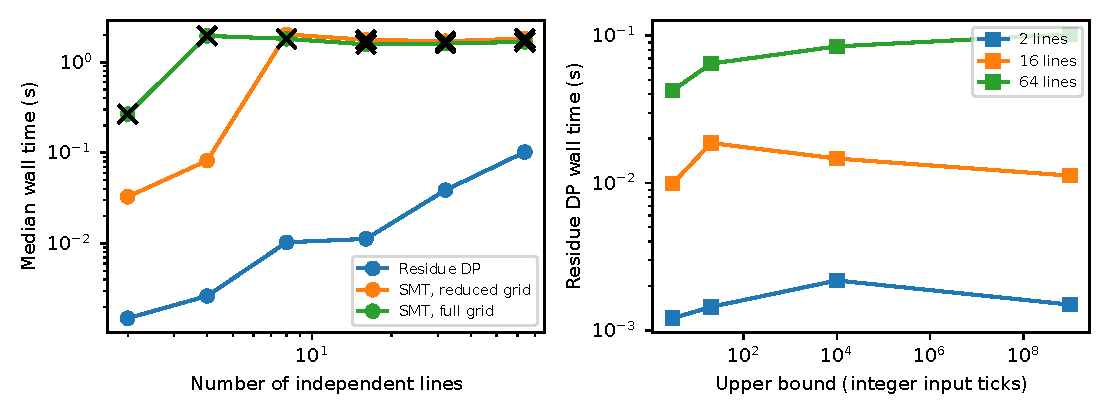
\includegraphics[width=\linewidth]{figures/scalability.pdf}
\caption{Saved scaling measurements. Left: median observed wall time over three runs at $U=10^9$; a cross marks a cell with at least one unfinished optimum computation. Such points measure time to the returned diagnostic and must not be interpreted as time to an exact answer. Right: DP timing as amount-window width changes for selected line counts. Coefficient denominators remain fixed within these curves.}
\label{fig:scaling}
\end{figure}

The largest DP median over the 24 cases is \DPMaxMedian\,ms (Figure~\ref{fig:scaling}). For the four-line, $U=10^9$ cell, the SMT medians are \ResidueFourMedian\,ms with structural reduction and \SMTFourMedian\,ms on the full grid. Reduction is not guaranteed to improve solver wall time: encoding and solver overhead can change its practical effect. Cells containing unfinished runs do not support exact-answer speedup ratios. The DP's finite residue work explains its weak dependence on interval width here, while larger denominators, coupled inputs, or branch structure require separate evaluation. Runtime and completion numbers are generated from the saved records through \texttt{result\_macros.tex}; reruns on another machine require reexamining the resulting plot and outcomes.

\paragraph{Independent scaling certificates and bound quality.}
Large boxes are not exhaustively enumerated. For each line, an independently executed Decimal table covers its feasible local period, or its whole interval when shorter; the sufficient periods of these benchmark rates are at most 20 ticks. Summing the local error minima and maxima gives a sound envelope for the total line error. The outer nearest-rounding error is at most $1/2$ cent. Since the final discrepancy is an integer number of cents, flooring this envelope supplies an independent integral upper bound. A DP-produced input is checked against every declared tick bound and replayed through Decimal. Its attained spread equals that independently derived upper bound in all 24 cases, certifying the maximum without assuming the DP's optimum calculation. The certificate values and witnesses are saved in \texttt{scaling\_ground\_truth.json}. This construction is specific to the saved scaling family, not an independent solver for arbitrary input programs.

The unrestricted nearest-even envelope is $\he(n/2)$ cents. At 64 lines and $U=3$, RoundGuard finds an attainable maximum of 27 cents, compared with the universal 32-cent envelope. At $U\ge20$, the 64-line maximum is 30 cents, leaving a two-cent gap even with complete local-period coverage; the heterogeneous line grids still exclude the universal endpoint. For 32 lines the corresponding maxima are 14 and 15 cents, compared with 16 cents universally. The saved upper-envelope certificate is tight in all scaling cases, whereas the universal envelope is strictly larger in ten of the 24 cases. This difference measures attainable-bound precision on declared grids, rather than a change in rounding semantics.

